\pdfminorversion=7
\documentclass[acmsmall,screen,review,anonymous]{acmart}

\usepackage{amsmath}
\usepackage{booktabs}
\usepackage{graphicx}
\usepackage{pifont}
\usepackage{tabularx}
\usepackage{tikz}
\usepackage{xspace}
\usepackage{xcolor}

\usetikzlibrary{arrows.meta, positioning, fit, calc, patterns, shapes.geometric}
% Shared TikZ style for the Backstop design figures (CASCADE look).
% The ACM template owns the document font; figure-local components reuse it.
% Every design figure is drawn at the text width (13.9 cm). The enclosing
% \resizebox keeps a scale close to one and the font sizes below are final.
\definecolor{panel}{gray}{0.94}
\definecolor{cyanp}{HTML}{BFE6EC}
\definecolor{peach}{HTML}{FBE1D2}
\definecolor{hot}{HTML}{E8735A}
\definecolor{gold}{HTML}{FFC000}
\definecolor{bluec}{HTML}{8FAADC}
\definecolor{greenc}{HTML}{A9D18E}
\definecolor{dred}{HTML}{C00000}
\definecolor{dblue}{HTML}{2E75B6}
\definecolor{navyf}{HTML}{1F3864}
\definecolor{okc}{HTML}{E2F0D9}
\definecolor{badc}{HTML}{F8D7D0}
\definecolor{debtc}{HTML}{FFE699}
\definecolor{aic}{HTML}{B4C7E7}
\definecolor{recc}{HTML}{F4B183}

\tikzset{
  layer/.style={draw=black!70, fill=panel, line width=0.5pt},
  frame/.style={draw=navyf, line width=0.7pt},
  sub/.style={draw=black!65, fill=white, line width=0.4pt},
  gpu/.style={draw=navyf, fill=cyanp, line width=0.5pt},
  comp/.style={draw=black, fill=white, line width=0.4pt, align=center,
               font=\bfseries\scriptsize, inner sep=1.5pt, minimum height=0.55cm},
  blk/.style={draw=black!70, line width=0.35pt, minimum width=0.5cm, minimum height=0.36cm,
              inner sep=0pt, font=\bfseries\scriptsize},
  free/.style={blk, pattern=north east lines, pattern color=black!55},
  cell/.style={draw=black!70, line width=0.35pt, anchor=north west, inner sep=0pt,
               minimum height=0.3cm, font=\scriptsize},
  hcell/.style={cell, fill=black!10, font=\bfseries\scriptsize},
  job/.style={draw=black!75, line width=0.4pt, inner sep=0pt, font=\bfseries\scriptsize},
  ttl/.style={font=\bfseries\small},
  pttl/.style={font=\bfseries\scriptsize},
  note/.style={font=\itshape\bfseries\scriptsize},
  inote/.style={font=\itshape\scriptsize},
  arr/.style={-{Latex[length=1.6mm]}, line width=0.8pt},
  darr/.style={{Latex[length=1.6mm]}-{Latex[length=1.6mm]}, line width=0.8pt},
  fat/.style={-{Triangle[length=2.2mm,width=3.4mm]}, line width=2.4pt},
  dfat/.style={{Triangle[length=1.8mm,width=3.0mm]}-{Triangle[length=1.8mm,width=3.0mm]},
               line width=2.0pt},
  guard/.style={draw=dred, dashed, line width=0.8pt},
  expiry/.style={draw=black, dotted, line width=0.9pt},
  num/.style={circle, fill=black, text=white, font=\bfseries\scriptsize,
              inner sep=0.6pt, minimum size=0.33cm},
  rnum/.style={num, fill=dred},
}

\newcommand{\SOFTWALLNAME}{Backstop}
\newcommand{\cmark}{\ding{51}}
\newcommand{\xmark}{\ding{55}}


\setcopyright{none}
\settopmatter{printacmref=true,printccs=true,printfolios=true}
\renewcommand\footnotetextcopyrightpermission[1]{}

\newcommand{\sys}{Backstop\xspace}
\newcommand{\NRx}{NeuralRx\xspace}

\begin{document}

\title[Backstop: Recovery-Safe GPU Sharing in AI-RAN]{Backstop: Recovery-Safe GPU Sharing Between
Neural Receivers and AI Inference in AI-RAN}

\acmConference[SIGMETRICS '27]{ACM SIGMETRICS 2027}{June 7--11, 2027}{Atlanta, Georgia, USA}
\acmYear{2027}

\begin{CCSXML}
<ccs2012>
 <concept>
  <concept_id>10010520.10010521.10010542</concept_id>
  <concept_desc>Computer systems organization~Real-time systems</concept_desc>
  <concept_significance>500</concept_significance>
 </concept>
 <concept>
  <concept_id>10003033.10003034.10003035</concept_id>
  <concept_desc>Networks~Network resources allocation</concept_desc>
  <concept_significance>300</concept_significance>
 </concept>
</ccs2012>
\end{CCSXML}

\ccsdesc[500]{Computer systems organization~Real-time systems}
\ccsdesc[300]{Networks~Network resources allocation}

\keywords{AI-RAN, GPU scheduling, neural receiver, MPS, admission control}

\begin{abstract}
AI-RAN servers run the uplink physical layer and AI inference on the same GPUs. Neural receivers decode
transport blocks (TBs) that the conventional receiver fails, but their value and their cost on a shared
GPU are not established. We compare public neural receivers with the cuPHY receiver at the same LDPC
iteration count and find that the real-time model helps only when the channels of paired users are
correlated, while a larger model decodes 15-67\% of the failed TBs on every channel we test. The larger
model takes 5.3~ms per slot, twice the uplink period. This paper presents \sys, which runs the larger model
only for failed TBs under a later deadline and grants AI inference in short pieces that keep both the
layer-1 deadline and the recovery deadline. On four A100 GPUs with 16 cells, \sys recovers 63-66\% of the
failed TBs on the low-correlation channel and 38\% with mixed channels. Under a load that changes every two
seconds, \sys serves 27.4k tokens/s while keeping 98.6\% of
the recoveries, 5.0$\times$ a fixed GPU share and 1.17$\times$ a share that follows the load, at the same
recovery level.
\end{abstract}

\maketitle

\section{Introduction}

Radio access networks (RANs) increasingly run baseband processing on GPUs, and AI-RAN platforms run radio
physical-layer (PHY) processing and AI inference on the same GPUs~\cite{aerial,yinyangran,interplay,distributedairan}.
To use the GPU time that radio processing leaves idle, these platforms add AI services, such as large
language model (LLM) inference, next to deadline-critical PHY tasks~\cite{caora,haf}. Neural receivers are a
PHY workload that these platforms now run on the GPU~\cite{aerial,nrxrt}. A neural receiver replaces channel estimation,
equalization, and demapping with a learned model and decodes transport blocks (TBs) that a conventional
receiver fails~\cite{deeprx,nrx5g,nrxrt}. Each TB that it decodes avoids a retransmission and frees an uplink
slot.

The challenge stems from two facts that we measure in this paper. First, the neural receiver that helps
is expensive. With the same number of LDPC iterations in both receivers, the real-time model of the public
NVlabs receivers~\cite{nrxrt,neuralrxsw} decodes more TBs than the cuPHY receiver only when the channels of
the paired users are correlated. The larger model decodes more TBs on every channel we test, and it takes
5.3~ms per slot against an uplink period of 2.5~ms. Thus, it cannot run for every slot. Second, the larger
model shares the GPU with the conventional receivers of all cells and with AI inference. NVIDIA
Multi-Process Service (MPS) caps the GPU threads of a process, but the cap is fixed when the process
starts~\cite{nvidiampS}. A cap that protects the radio work at full load leaves the GPU idle when the load
drops, and a cap that fits a light load delays the radio work at full load.

\begin{table}[t]
\caption{What the closest public designs run on the shared GPU.}
\label{tab:closest}
\footnotesize
\begin{tabularx}{\linewidth}{@{}>{\raggedright\arraybackslash}p{0.25\linewidth}>{\raggedright\arraybackslash}p{0.31\linewidth}>{\raggedright\arraybackslash}X@{}}
\toprule
System & Radio work on the GPU & How AI shares the GPU \\
\midrule
YinYangRAN, CloudRIC, Concordia & LDPC decoding or queued PHY jobs & GPU share or reserved capacity, changed at intervals of one second or more \\
DARIS, REEF, XSched, nvtaskset & None; generic GPU tasks & Kernel, context, or partition priority without radio deadlines \\
ARCHES, OCUDU, neural receivers & Neural channel estimator or neural receiver & No AI workload on the same GPU \\
\sys & Conventional receiver for every TB and a neural receiver for failed TBs & AI pieces granted against the layer-1 deadline and the recovery deadline \\
\bottomrule
\end{tabularx}
\end{table}

Existing systems cover one side of this problem. As Table~\ref{tab:closest} summarizes, vRAN and AI-RAN
resource managers~\cite{yinyangran,cloudric,concordia,interplay,caora,haf,distributedairan} share GPUs
between radio processing and other workloads by a GPU share or by reserved capacity, and their radio work is
LDPC decoding or the conventional PHY. GPU scheduling systems~\cite{daris,reef,xsched,nvtaskset} prioritize
or preempt GPU kernels and contexts without radio deadlines. Neural receiver studies and PHY
platforms~\cite{deeprx,nrx5g,nrxrt,arches,ocudu} design the receiver or switch between PHY models, and they
do not share the GPU with an AI workload. However, none of them runs a neural receiver next to AI inference
on one GPU while keeping the deadlines of both radio paths.

In this paper, we present \sys, a GPU sharing scheme for AI-RAN servers that uses a neural receiver as a
second receiver for the TBs the conventional receiver fails. Specifically, \sys introduces 1) a recovery
path that sends a failed TB to the neural receiver only when the number of failed code blocks predicts a
successful decode, 2) two deadlines per TB, the layer-1 deadline for the conventional receiver and a later
recovery deadline before the retransmission is scheduled, and 3) AI admission in bounded pieces, where the
controller allows a piece only if every running and waiting radio job still meets its deadline. Our
evaluation on four A100 GPUs with 16-32 cells, the cuPHY receiver, the public NVlabs neural receivers, and
Qwen2.5 prefill requests shows that \sys recovers 63-66\% of the TBs the conventional receiver fails on the
low-correlation channel and 38\% with mixed channels. With
mixed channels and a load that alternates between full and half every two seconds, \sys serves 27.4k
tokens/s within the 200~ms limit and keeps 98.6\% of the recoveries. A fixed 10\% GPU share keeps the same
recoveries at 5.5k tokens/s, and a share that switches between 10\% and 50\% with the load, with no
switching cost, reaches 23.5k tokens/s. When the neural receiver load is light, a fixed share serves more AI
than \sys, and we report those settings as well.

\section{Background and Motivation}

\subsection{AI-RAN on shared GPUs}

An AI-RAN server decodes the uplink of many cells on GPUs and serves AI requests with the GPU time that is
left~\cite{aerial,distributedairan}.

\noindent\textbf{Uplink Timeline.} With the TDD pattern DDDSU at 30~kHz subcarrier spacing, every cell has
one uplink slot per 2.5~ms. The received samples of a slot are ready 0.5~ms after the slot starts, and the
layer-1 result is due 4.5~ms after the slot starts, which leaves 4.0~ms for decoding. A TB that fails is
retransmitted three uplink slots later, 7.5~ms after the original slot: the grant goes out in the
special slot before that uplink slot with a scheduling offset of one slot, which the PUSCH preparation time
of 12 symbols allows~\cite{ts38214}.

\noindent\textbf{GPU Sharing.} MPS runs the processes of one GPU concurrently and caps the active threads of
each process~\cite{nvidiampS}. YinYangRAN changes the share between LDPC decoding and other workloads with
a learned predictor at intervals of at least one second~\cite{yinyangran}, and CloudRIC pools GPUs for LDPC
decoding across distributed units~\cite{cloudric}. The share of an MPS client cannot change after the client
starts. Therefore, a system that follows the load must restart the client or keep one loaded client per
share.

\subsection{When does a neural receiver help?}

We compare the public NVlabs neural receivers~\cite{nrx5g,nrxrt,neuralrxsw} with the cuPHY PUSCH
receiver~\cite{aerial} on the same received slots. Two users transmit on the same 273 PRBs with 16QAM, and
the base station has four antennas. The slots come from the NVlabs link simulation~\cite{sionna}; cuPHY
decodes them with MMSE equalization and time interpolation.

\noindent\textbf{Same LDPC Effort.} A receiver comparison is valid only when both receivers run the same
number of LDPC iterations. cuPHY uses 10 iterations for the TB sizes in our setup, and the evaluation code
of the neural receivers uses 20. With 10 against 20 iterations, the real-time model appears to decode
25-35\% of the TBs that cuPHY fails on the low-correlation channel. With 20 iterations on both sides, the
figure is 2\%. Raising cuPHY from 10 to 20 iterations alone recovers 152 of 158 failed single-user TBs, at
15-19\% more receiver time for TBs of 13-20 code blocks. Therefore, every result in this paper uses 20
iterations in both receivers. Table~\ref{tab:receivers} shows the comparison.

\begin{table}[t]
\caption{TBs decoded at 20 LDPC iterations in both receivers. The percentage is the share of the TBs cuPHY
fails that the neural receiver decodes; the time is the GPU time of the model alone.}
\label{tab:receivers}
\footnotesize
\begin{tabular}{@{}lrrll@{}}
\toprule
Channel of the two users & TBs & cuPHY & Real-time model (1.35~ms) & Larger model (4.29~ms) \\
\midrule
Low correlation, 2-3~dB & 600 & 515 & 484 (2\%) & 572 (67\%) \\
Urban micro, 1-6~dB & 600 & 425 & 420 (2\%) & 451 (15\%) \\
Medium correlation, 8-18~dB & 600 & 321 & 372 (21\%) & not measured \\
High correlation, 10-16~dB & 1,400 & 946 & 1,099 (38\%) & 1,159 (51\%) \\
\bottomrule
\end{tabular}
\end{table}

\noindent\textbf{The Model That Helps Is Too Slow for Every Slot.} The real-time model decodes more TBs
than cuPHY only when the channels of the two users are correlated. The larger model decodes more TBs on all
three channels and loses none of the TBs that cuPHY decodes on two of them. It takes 5.3~ms per slot alone
and 6.3~ms next to the cell workload, against an uplink period of 2.5~ms; cuPHY takes 0.8-0.9~ms. When we
send every slot of four cells to the larger model, 61\% of the slots find no free GPU in time and 89.4\% of
the TBs are decoded. When we send only the TBs that cuPHY fails, the neural receiver runs for 25\% of the
slots, the decode result is the same offline, and 94.5-95.1\% of the TBs are decoded in the timed system.

\noindent\textbf{Failed Code Blocks Predict the Outcome.} The conventional receiver reports how many code
blocks of a TB failed. On the urban micro channel, 87\% of the failed TBs have every code block failed and
the neural receiver decodes 2\% of them. It decodes 93\% of the TBs in slots with at most nine failed code
blocks. On the low-correlation channel, it decodes 97\% of the failed TBs in slots with one to three failed
code blocks and 30\% in slots with ten or more.

This motivates \sys's design: run the larger model only for failed TBs that it is likely to decode, give
that run a deadline later than the layer-1 deadline, and admit AI only where both deadlines hold.

\section{Backstop Design}

\subsection{Overall architecture}

\begin{figure}[t]
\centering
\resizebox{\linewidth}{!}{% Overall architecture of slot-scale Backstop, with the values of the run in Fig. 2 (cell 3, slot 547).
% Processes and GPU placement: launch_slot.py; state rows: slot_state.py; steps: controller3.py.
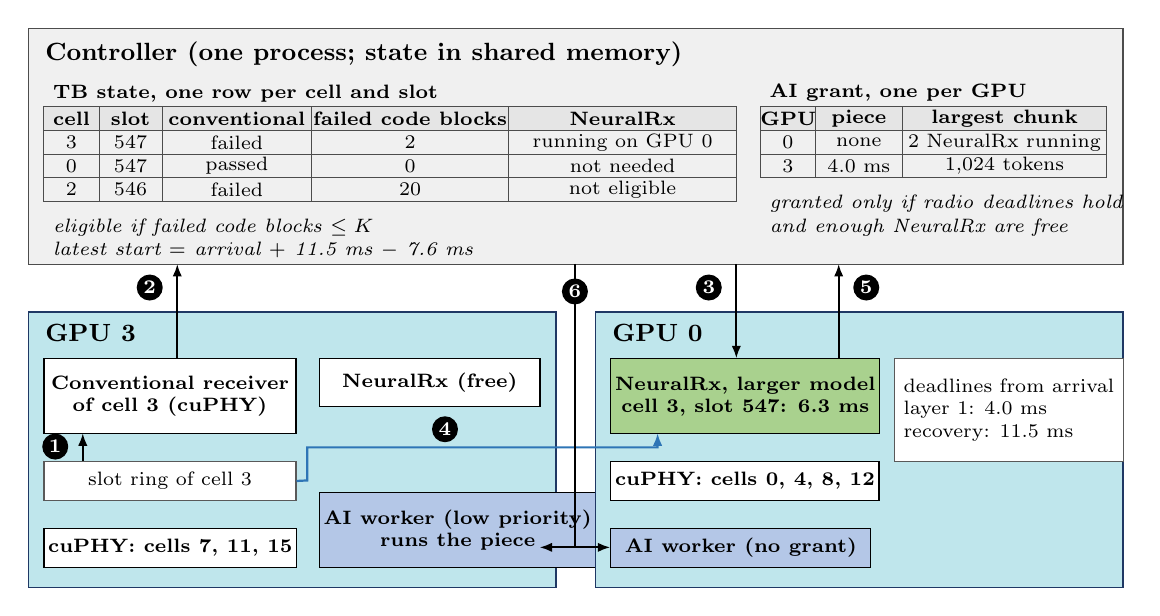
\begin{tikzpicture}[x=1cm, y=1cm, font=\scriptsize]
  % ---------------- controller ----------------
  \node[layer, anchor=north west, minimum width=13.9cm, minimum height=3.0cm] (ctl) at (0,0) {};
  \node[ttl, anchor=north west] at (0.1,-0.05) {Controller (one process; state in shared memory)};
  \node[pttl, anchor=north west] at (0.2,-0.6) {TB state, one row per cell and slot};
  \foreach \x/\w/\h in {0.2/0.7/cell, 0.9/0.8/slot, 1.7/1.9/conventional, 3.6/2.5/failed code blocks, 6.1/2.9/NeuralRx}
    \node[hcell, minimum width=\w cm] at (\x,-1.0) {\h};
  \foreach \y/\a/\b/\c/\d/\e in {-1.3/3/547/failed/2/running on GPU 0, -1.6/0/547/passed/0/not needed, -1.9/2/546/failed/20/not eligible}
  {
    \node[cell, minimum width=0.7cm] at (0.2,\y) {\a};
    \node[cell, minimum width=0.8cm] at (0.9,\y) {\b};
    \node[cell, minimum width=1.9cm] at (1.7,\y) {\c};
    \node[cell, minimum width=2.5cm] at (3.6,\y) {\d};
    \node[cell, minimum width=2.9cm] at (6.1,\y) {\e};
  }
  \node[inote, anchor=north west] at (0.2,-2.3) {eligible if failed code blocks $\le K$};
  \node[inote, anchor=north west] at (0.2,-2.6) {latest start $=$ arrival $+$ 11.5 ms $-$ 7.6 ms};
  \node[pttl, anchor=north west] at (9.3,-0.6) {AI grant, one per GPU};
  \foreach \x/\w/\h in {9.3/0.7/GPU, 10.0/1.1/piece, 11.1/2.6/largest chunk}
    \node[hcell, minimum width=\w cm] at (\x,-1.0) {\h};
  \foreach \y/\a/\b/\c in {-1.3/0/none/2 NeuralRx running, -1.6/3/4.0 ms/{1,024 tokens}}
  {
    \node[cell, minimum width=0.7cm] at (9.3,\y) {\a};
    \node[cell, minimum width=1.1cm] at (10.0,\y) {\b};
    \node[cell, minimum width=2.6cm] at (11.1,\y) {\c};
  }
  \node[inote, anchor=north west] at (9.3,-2.0) {granted only if radio deadlines hold};
  \node[inote, anchor=north west] at (9.3,-2.3) {and enough NeuralRx are free};

  % ---------------- GPU 3 ----------------
  \node[gpu, anchor=north west, minimum width=6.7cm, minimum height=3.5cm] (g3) at (0,-3.6) {};
  \node[ttl, anchor=north west] at (0.1,-3.65) {GPU 3};
  \node[comp, anchor=north west, minimum width=3.2cm, minimum height=0.95cm] (c3) at (0.2,-4.2)
    {Conventional receiver\\of cell 3 (cuPHY)};
  \node[sub, anchor=north west, minimum width=3.2cm, minimum height=0.5cm, align=center] (ring3) at (0.2,-5.5)
    {slot ring of cell 3};
  \node[comp, anchor=north west, minimum width=3.2cm, minimum height=0.5cm] (c3b) at (0.2,-6.35)
    {cuPHY: cells 7, 11, 15};
  \node[comp, anchor=north west, minimum width=2.8cm, minimum height=0.6cm] (n3) at (3.7,-4.2) {NeuralRx (free)};
  \node[comp, anchor=north west, minimum width=2.8cm, minimum height=0.95cm, fill=aic] (a3) at (3.7,-5.9)
    {AI worker (low priority)\\runs the piece};

  % ---------------- GPU 0 ----------------
  \node[gpu, anchor=north west, minimum width=6.7cm, minimum height=3.5cm] (g0) at (7.2,-3.6) {};
  \node[ttl, anchor=north west] at (7.3,-3.65) {GPU 0};
  \node[comp, anchor=north west, minimum width=3.3cm, minimum height=0.95cm, fill=greenc] (n0) at (7.4,-4.2)
    {NeuralRx, larger model\\cell 3, slot 547: 6.3 ms};
  \node[comp, anchor=north west, minimum width=3.3cm, minimum height=0.5cm] (c0) at (7.4,-5.5)
    {cuPHY: cells 0, 4, 8, 12};
  \node[comp, anchor=north west, minimum width=3.3cm, minimum height=0.5cm, fill=aic] (a0) at (7.4,-6.35)
    {AI worker (no grant)};
  \node[sub, anchor=north west, minimum width=2.7cm, minimum height=1.3cm, align=left] (leg) at (11.0,-4.2)
    {deadlines from arrival\\layer 1: 4.0 ms\\recovery: 11.5 ms};

  % ---------------- arrows and steps ----------------
  \draw[arr] (0.7,-5.5) -- (0.7,-5.15);
  \node[num] at (0.35,-5.32) {1};
  \draw[arr] (1.9,-4.2) -- (1.9,-3.0);
  \node[num] at (1.55,-3.3) {2};
  \draw[arr] (9.0,-3.0) -- (9.0,-4.2);
  \node[num] at (8.65,-3.3) {3};
  \draw[arr, dblue] (ring3.east) -- (3.55,-5.75) -- (3.55,-5.33) -- (8.0,-5.33) -- (8.0,-5.15);
  \node[num] at (5.3,-5.1) {4};
  \draw[arr] (10.3,-4.2) -- (10.3,-3.0);
  \node[num] at (10.65,-3.3) {5};
  \draw[arr] (6.95,-3.0) -- (6.95,-6.6) -- (6.5,-6.6);
  \draw[arr] (6.95,-6.6) -- (7.4,-6.6);
  \node[num] at (6.95,-3.35) {6};
\end{tikzpicture}
}
\caption{Overall architecture of \sys with the values of one recovery in a measured run (two of the four
GPUs are shown). Numbers mark the steps of the text.}
\label{fig:architecture}
\end{figure}

\sys runs four kinds of processes on each server (Figure~\ref{fig:architecture}). A conventional receiver
process per cell decodes the TBs of its cell with cuPHY every 2.5~ms. A neural receiver process per GPU
decodes one TB at a time. An AI worker per GPU runs AI inference in pieces. One controller assigns failed TBs
to neural receivers, grants AI pieces, and places AI requests on GPUs. All processes read one shared state
in memory and one clock.

The steps for one slot are as follows. \ding{202}~The samples of a slot arrive in the slot ring of the cell,
which stays in the GPU memory of its conventional receiver, and cuPHY decodes them. \ding{203}~The receiver
writes the CRC result and the number of failed code blocks to the TB state. \ding{204}~The controller
assigns an eligible failed TB to a free neural receiver before the latest start time of the TB.
\ding{205}~Every neural receiver process maps the slot rings of all cells. Thus, the neural receiver copies
the slot from the GPU of the cell and decodes it on its own GPU. \ding{206}~A result that arrives before
the recovery deadline cancels the retransmission. \ding{207}~In every round the controller writes one AI
grant per GPU, and the AI worker runs only inside the granted piece.

\subsection{Recovery path}

\noindent\textbf{Two Deadlines.} Every TB has a layer-1 deadline of 4.0~ms after its samples arrive, which
the conventional receiver must meet. A TB that fails has a \emph{recovery deadline}: if the neural receiver
decodes it before this deadline, the retransmission is cancelled. A recovery deadline of 6.5~ms keeps the
retransmission slot of the conventional path. The larger model does not fit into 6.5~ms, and \sys uses
11.5~ms, which delays the retransmission of a TB that is not recovered by two uplink slots (5~ms).

\noindent\textbf{Which TBs Are Recovered.} A failed TB becomes a candidate only if its slot has at most $K$
failed code blocks. The controller computes the latest start time of a candidate as its arrival plus the
recovery deadline minus the time bound of the neural receiver. It assigns candidates in order of latest
start time to a free neural receiver, preferring a GPU with no other neural receiver running and no AI piece
running. A candidate that passes its latest start time is dropped and its TB is retransmitted. A neural
receiver result counts only if the CRC passes, the payload is correct, and the run ends before the recovery
deadline.

\subsection{AI admission in bounded pieces}

\noindent\textbf{AI Units.} The AI worker splits the prefill of an LLM request into units of one layer over
a chunk of 128, 512, or 1,024 tokens, each compiled as one GPU graph with a measured time bound. A larger
chunk is faster per token and holds the GPU longer once it starts.

\noindent\textbf{Grants.} The AI worker runs under an MPS share of 70\% and submits units only inside a
piece that the controller grants. For each GPU the controller picks the largest chunk size $c$ that meets
all of the following and grants a piece of at most 4~ms:
\begin{itemize}
\item \emph{Running neural receiver.} For every neural receiver running on this GPU, its start time plus
$B(c)$ is before its recovery deadline, where $B(c)$ is the time bound of the neural receiver next to AI
units of size $c$.
\item \emph{Conventional receivers.} If size $c$ is not allowed next to the conventional receivers, no cell
of this GPU is decoding and the piece ends before the next slot arrives.
\item \emph{Neural receiver about to start.} If a TB of this GPU may still become a candidate, the piece
ends before the latest start time of that TB under $B(c)$.
\item \emph{Waiting candidates.} No candidate is waiting for a free neural receiver.
\end{itemize}
If no size meets the conditions, the GPU gets no AI in this round. The worker keeps the chunk size of a
request stable by choosing the largest size that was allowed for most of the last 20~ms.

\begin{figure}[t]
\centering
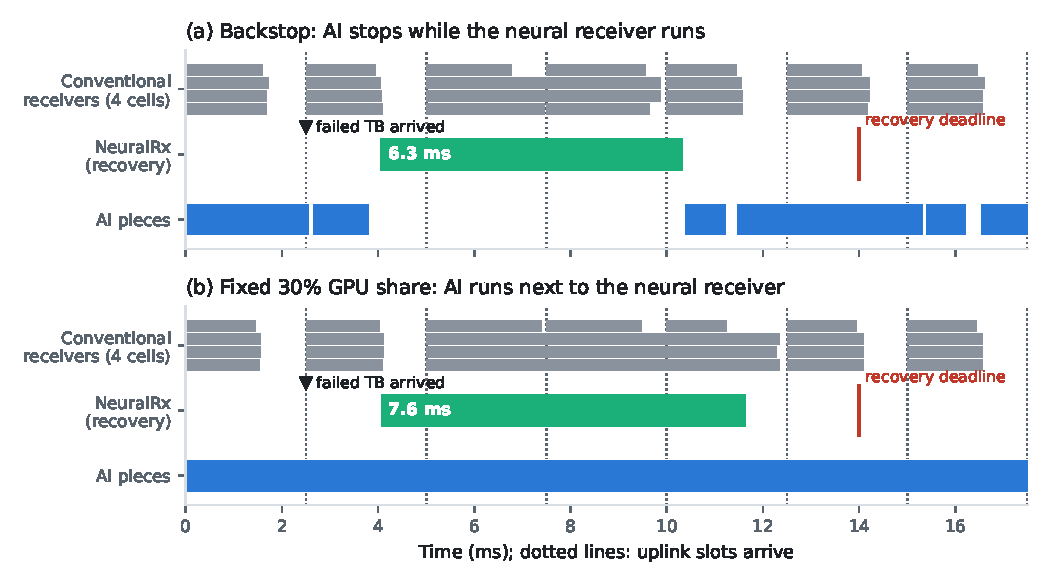
\includegraphics[width=0.9\linewidth]{figures/timeline_one_gpu.pdf}
\caption{Measured timeline of GPU~0 around one recovery (the run of Figure~\ref{fig:architecture}, same
seed for both policies). Bars show when each job runs.}
\label{fig:timeline}
\end{figure}

Figure~\ref{fig:timeline} shows the effect on a measured run. Under \sys, the AI worker stops before the
neural receiver starts, the neural receiver finishes in 6.3~ms, and the AI worker resumes after it. Under a
fixed 30\% share, AI runs next to the neural receiver, which takes 7.6~ms, and next to the conventional
receivers, which finish later.

\noindent\textbf{AI Requests.} The controller predicts when a new request would finish from the tokens that
wait on each GPU and the recent prefill rate of that GPU. It places the request on the GPU that finishes it
first and rejects it if no GPU finishes it within the limit. Every baseline uses the same placement and
rejection.

\subsection{Time bounds and implementation}

The bounds come from measurements of the 99.9th percentile on the evaluation hardware with all cells
running. With 16 cells, the larger neural receiver takes 6.3~ms at the median and the bound is 7.6~ms alone
and 9.8-10.3~ms next to AI units. The neural receiver path is the public TensorRT export of the NVlabs
model followed by rate recovery, LDPC decoding, and CRC from cuPHY. We replace the least-squares channel
estimation call with one multiplication of the pilot samples and call the cuPHY bit-level functions on
buffers allocated once, which shortens the path of the real-time model from 3.08 to 2.36~ms with the same
decoded TBs. The run-time path of the real-time model agrees with the NVlabs evaluation on 794 of 800 TBs.
\sys is 2.9k lines of Python over cuPHY, TensorRT, and PyTorch.

\section{Evaluation}

\subsection{Evaluation setup}

\noindent\textbf{Hardware.} One node with four NVIDIA A100 80~GB GPUs under MPS and 64 CPU cores.

\noindent\textbf{Scope.} All measurements are end-to-end runs on the GPUs: cuPHY decodes every TB, the
neural receiver decodes real received slots, and the AI worker runs real prefill. The slots are generated in
advance; there is no radio unit and no layer-2 stack.

\noindent\textbf{Workloads.} Sixteen cells run on four GPUs, four per GPU, unless stated. One cell per GPU
carries two users on the same 273 PRBs (16QAM, 20 code blocks per slot); the other cells carry one user
with two layers. The two-user slots come from three channels of the NVlabs link simulation: low
correlation at 2-3~dB, high correlation at 13-16~dB, and urban micro~\cite{tr38901} at 4-6~dB. Both
receivers run 20 LDPC iterations, the neural receiver is the larger NVlabs model, $K=9$ with mixed channels,
and the recovery deadline is 11.5~ms. AI requests are Qwen2.5-1.5B~\cite{qwen25} prefill requests of up to
1,024 tokens with a 200~ms limit, offered at 32 requests/s per GPU. A request that finishes after the limit
does not count. Runs last 10-20~s; values are means over seeds.

\noindent\textbf{Baselines.} \emph{Fixed share} gives the AI worker a fixed MPS share and no grants.
\emph{Share that follows the load} keeps one AI worker per share loaded on every GPU and makes the
low-share worker active while the GPU is at full load and the high-share worker otherwise. It has no
switching cost, the waiting requests pass to the active worker, and we run it with the load known at once
and known one second late, the minimum reconfiguration interval of YinYangRAN~\cite{yinyangran}. All
policies use the same recovery path, the same AI requests, and the same placement and rejection of AI
requests. We report the recoveries of a run as a share of the recoveries of the run without AI on the same
seed.

\subsection{AI served under a changing load}

\begin{figure}[t]
\centering
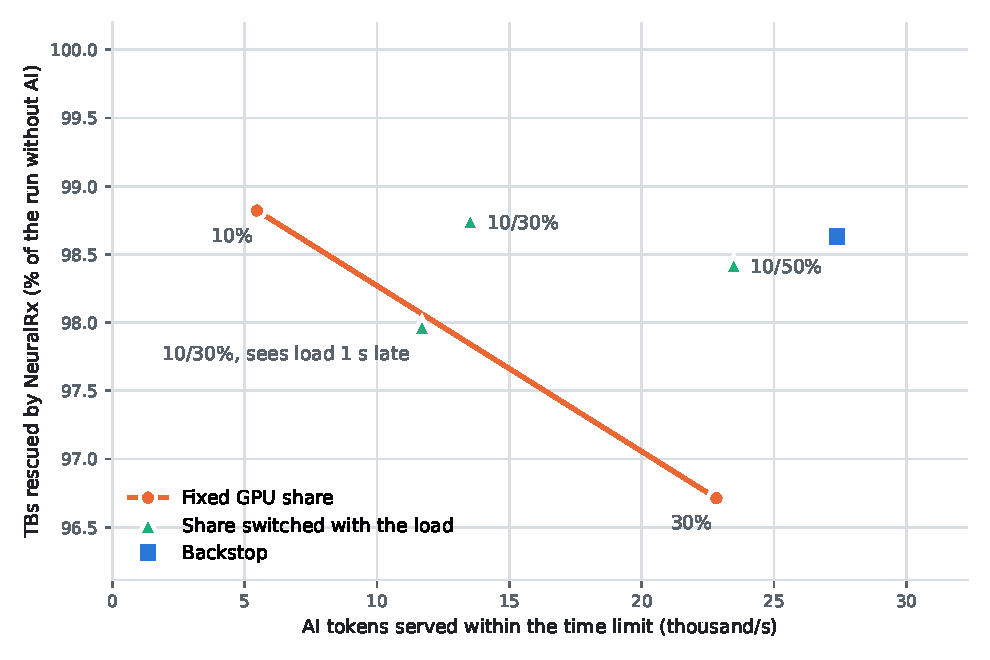
\includegraphics[width=0.62\linewidth]{figures/changing_load_16cells.pdf}
\caption{AI served and recoveries kept when the radio load alternates between full and half every 2~s
(16 cells, mixed channels, five seeds). Labels give the MPS shares.}
\label{fig:changing}
\end{figure}

\begin{table}[t]
\caption{Changing load, 16 cells, mixed channels, five seeds (range over seeds in parentheses).}
\label{tab:changing}
\footnotesize
\begin{tabular}{@{}lll@{}}
\toprule
Policy & AI tokens/s within 200~ms & Recoveries kept \\
\midrule
\sys & 27.4k (26.0-28.5k) & 98.6\% (97.6-99.3\%) \\
Fixed 10\% & 5.5k (5.3-5.6k) & 98.8\% (97.4-99.8\%) \\
Fixed 30\% & 22.8k (21.9-23.5k) & 96.7\% (95.5-98.6\%) \\
Share follows load, 10/30\% & 13.5k (12.6-14.6k) & 98.7\% (97.7-99.6\%) \\
Share follows load, 10/50\% & 23.5k (22.9-24.6k) & 98.4\% (97.3-99.3\%) \\
Share follows load, 10/30\%, 1~s late & 11.7k (11.5-11.8k) & 98.0\% (96.6-99.2\%) \\
\bottomrule
\end{tabular}
\end{table}

The radio load alternates every two seconds between full load and each cell active with probability 0.5.
Figure~\ref{fig:changing} and Table~\ref{tab:changing} show AI served against recoveries kept. \sys serves
27.4k tokens/s and keeps 98.6\% of the recoveries. The fixed 10\% share keeps 98.8\% and serves 5.5k
tokens/s, 5.0$\times$ less. The fixed 30\% share serves 22.8k tokens/s and loses 3.3\% of the recoveries,
2.4$\times$ more than \sys. The share that follows the load serves 13.5-23.5k tokens/s at the same recovery
level, 1.17-2.0$\times$ less than \sys, and 11.7k tokens/s when it sees the load one second late. \sys
achieves this by granting AI during full load whenever no neural receiver runs on that GPU: it serves 18.8k
tokens/s in the full-load phases, while the share that follows the load drops to its 10\% share there and
serves 2.4-2.7k tokens/s. Layer-1 misses in the full-load phases are 0.03-0.04\% of the TBs for every
policy.

With 32 cells and a load that alternates between half and a quarter, the order is the same. \sys serves
26.4k tokens/s and keeps 99.4\% of the recoveries. The fixed 10\% share serves 5.3k tokens/s at 99.4\%, the
fixed 30\% share 22.0k at 97.7\%, and the share that follows the load 22.7k at 99.0\% with shares of 10 and
50\%.

\subsection{AI served at a steady full load}

\begin{table}[t]
\caption{Steady full load, 16 cells. Mixed channels with five seeds; one channel with three seeds.}
\label{tab:steady}
\footnotesize
\begin{tabular}{@{}lllll@{}}
\toprule
 & \multicolumn{2}{c}{Mixed channels} & \multicolumn{2}{c}{Low correlation, $K=20$} \\
Policy & Tokens/s & Recoveries kept & Tokens/s & Recoveries kept \\
\midrule
\sys & 22.7k & 97.9\% & 12.6k & 98.2\% \\
Fixed 10\% & 5.0k & 98.3\% & 4.4k & 97.5\% \\
Fixed 20\% & 10.8k & 97.3\% & 9.0k & 96.4\% \\
Fixed 30\% & 20.9k & 95.1\% & 15.9k & 93.8\% \\
Fixed 50\% & 36.3k & 91.9\% & 25.9k & 87.0\% \\
\bottomrule
\end{tabular}
\end{table}

Table~\ref{tab:steady} shows the steady full load. With mixed channels, \sys serves 22.7k tokens/s and
keeps 97.9\% of the recoveries. The fixed 10\% share keeps 98.3\% at 5.0k tokens/s, and the fixed 30\%
share serves 20.9k tokens/s and keeps 95.1\%. With the low-correlation channel alone, every failed TB goes
to the neural receiver and the neural receiver runs for 25\% of the slots. \sys serves 12.6k tokens/s at
98.2\%; a fixed share must drop to 10\% to keep 97.5\%, where it serves 4.4k tokens/s. At the same AI
served, \sys keeps 2-3 percentage points more recoveries than the fixed shares. The high-correlation channel
gives the same picture: \sys serves 11.9k tokens/s at 99.5\%, and the fixed 10\% share 4.2k at 99.3\%.
The fixed 50\% share misses the layer-1 deadline for 0.12-0.29\% of the TBs, against 0.04-0.06\% for \sys.

\subsection{Choosing the TBs to recover}

On the urban micro channel, sending every failed TB to the neural receiver takes 4,891-4,926 runs and
recovers 663-757 TBs without AI. Sending only the TBs of slots with at most nine failed code blocks takes
651-777 runs and recovers 589-746 TBs: 85\% fewer runs for 5\% fewer recoveries. With AI, \sys serves 6.4k
tokens/s without the rule and 33.6k with it. On the low-correlation channel with eight two-user cells, the
neural receivers cannot take every failed TB. Sending only slots with at most three failed code blocks
removes 40\% of the runs and 22\% of the recoveries, raises the recoveries per run from 0.77 to 0.99, and
raises the AI that \sys serves from 2.2k to 12.4k tokens/s.

\subsection{Where recoveries are lost}

We classify every recovery that a policy loses against the run without AI. With the larger model and a
fixed 50\%, 70\%, or 100\% share, 10.8\%, 12.8\%, and 18.6\% of the recoveries are lost because no neural
receiver is free before the latest start time, and 4.9\%, 13.9\%, and 39.1\% because the neural receiver
finishes after the recovery deadline. \sys loses 3.4\% to busy neural receivers and none to late results.
With a 6.5~ms recovery deadline and the real-time model, the losses of the fixed shares are a conventional
result that arrives after the latest start time (5-25\%), because AI delays the conventional receiver by
0.2-0.4~ms, and a busy neural receiver (5-13\%). Late results stay below 4\%.

\subsection{Where a fixed share is enough}

\sys's advantage needs a neural receiver load that fills a large part of the GPU. With the real-time model
(2.7~ms per recovery) and the 11.5~ms recovery deadline, a fixed 70\% share loses 1.5\% of the recoveries
and serves 43.1k tokens/s, against 34.7k tokens/s at 99.8\% for \sys. With the urban micro channel and the
failed-code-block rule, 5\% of the slots need the neural receiver, and a fixed 50\% share serves 46.0k
tokens/s against 33.6k for \sys at the same 99.8\%. At a steady half load, a fixed 30\% share keeps
99.3-99.5\% of the recoveries and serves 21.9-24.6k tokens/s, against 29.2k at 99.9\% for \sys. A fixed share
that fits one load does not fit another: the share that keeps the recoveries at full load is 10\%.

\section{Related Work}

\noindent\textbf{GPU sharing in vRAN and AI-RAN.} YinYangRAN~\cite{yinyangran} multiplexes LDPC decoding
with other workloads by MPS shares that a learned predictor changes at intervals of at least one second.
CloudRIC~\cite{cloudric} pools accelerators for LDPC decoding, and Concordia~\cite{concordia} reserves
capacity for vRAN tasks. AI-RAN studies~\cite{interplay,caora,haf,distributedairan} place AI and RAN
workloads across servers. Their radio work has one deadline and no second receiver. \sys adds a recovery
path with its own deadline and grants AI against both.

\noindent\textbf{GPU scheduling.} DARIS, REEF, XSched, and nvtaskset~\cite{daris,reef,xsched,nvtaskset}
schedule GPU stages, kernels, or contexts by priority. They have no notion of a TB that may still need a
neural receiver. \sys decides from the state of each TB.

\noindent\textbf{Neural receivers.} DeepRx~\cite{deeprx} and the NVlabs receivers~\cite{nrx5g,nrxrt} design
and train neural receivers, ARCHES~\cite{arches} switches between an AI channel estimator and a conventional
one, and OCUDU~\cite{ocudu} exposes timing classes in the distributed unit. These works report receiver
gains against their own baselines. We compare at equal LDPC effort with a production receiver and study the
neural receiver as a workload that shares the GPU with AI.

\section{Limitations}

The channels are the synthetic channels of the public NVlabs configuration. The larger model allows four to
five cells per GPU at full load; 32 cells run when half of the cells are idle. The recovery deadline follows
from the TDD pattern and the PUSCH preparation time~\cite{ts38214} and is not validated with a layer-2
stack; an 11.5~ms deadline delays the retransmission of an unrecovered TB by 5~ms. The share that follows the
load is our implementation with two shares and no load predictor. Layer-1 misses are 0.02-0.06\% of the TBs
for \sys and for the run without AI, which reflects the Python prototype and not a bound.

\section{Conclusion}

A neural receiver that decodes more TBs than a production receiver at equal LDPC effort takes twice the
uplink period. \sys runs it only for the TBs the conventional receiver fails and that it is likely to
decode, under a recovery deadline, and grants AI inference in pieces that keep the layer-1 deadline and the
recovery deadline. Under a changing load with mixed channels, \sys serves 27.4k tokens/s while keeping
98.6\% of the recoveries, 5.0$\times$ a fixed GPU share and 1.17$\times$ a share that follows the load.

\bibliographystyle{ACM-Reference-Format}
\bibliography{references}

\end{document}
